\documentclass[FM,DP]{tulthesis}

\usepackage{polyglossia}
\setdefaultlanguage{czech}
\usepackage{fontspec}
\usepackage{xunicode}
\usepackage{xltxtra}
\setsansfont[Mapping=tex-text,BoldFont={* Bold},Numbers=OldStyle]{Myriad Pro}
\usepackage{hyperref}
\hypersetup{colorlinks=true, linkcolor=tul, urlcolor=tul, citecolor=tul}
\usepackage{graphicx}
\usepackage{listings}
\usepackage[toc,page]{appendix}
\usepackage{amsmath}
\usepackage{amssymb}
\usepackage{minted}

%\usepackage{xpatch,letltxmacro}
%\LetLtxMacro{\cminted}{\minted}
%\let\endcminted\endminted
%\xpretocmd{\cminted}{\RecustomVerbatimEnvironment{Verbatim}{BVerbatim}{}}{}{}

\newcommand{\argument}[1]{{\ttfamily\color{\tulcolor}#1}}
\newcommand{\prikaz}[1]{\argument{\textbackslash #1}}
\newenvironment{myquote}{\begin{list}{}{\setlength\leftmargin\parindent}\item[]}{\end{list}}
%\newenvironment{listing}{\begin{myquote}\color{\tulcolor}}{\end{myquote}}
\sloppy


%%%%%%%%%%%%%%%%%%%%%%%%%%%%
\TULtitle{Vyhledávání jako služba}{Search as a Service}
\TULprogramme{Aplikovaná informatika}{Applied Informatics}
\TULbranch{Informační systémy a technologie}{Information Technologies}
\TULauthor{Bc. Luděk Veselý}
\TULsupervisor{Prof. Ing. Zdeněk Molnár, CSc.}
\TULyear{2017}


%%%%%%%%%%%%%%%%%%%%%%%%%%%%
\begin{document}
\ThesisStart{male}


%%%%%%%%%%%%%%%%%%%%%%%%%%%%
\begin{abstractCZ}
Tato diplomová práce popisuje návrh a tvorbu fulltextového vyhledávání poskytovaného jako služba.
\end{abstractCZ}

\begin{klicovaslovaCZ}
Fulltext, Elasticsearch
\end{klicovaslovaCZ}

\vspace{2cm}

\begin{abstractEN}
This diploma thesis describes creation of fulltext search service.
\end{abstractEN}

\begin{klicovaslovaEN}
Fulltext, Elasticsearch
\end{klicovaslovaEN}


%%%%%%%%%%%%%%%%%%%%%%%%%%%%
\begin{acknowledgement}
Rád bych poděkoval Ing. Ivanovi Jelínkovi za rady a pomoc při řešení.
\end{acknowledgement}


%%%%%%%%%%%%%%%%%%%%%%%%%%%%
\tableofcontents
\clearpage


%%%%%%%%%%%%%%%%%%%%%%%%%%%%
\begin{abbrList}
\textbf{URL} & 
Uniform Resource Locator, adresa dokumentu na webu\\
\textbf{XML} & 
Extensible Markup Language, značkovací jazyk\\
\textbf{EAN} & 
European Article Number, mezinárodní číselná identifikace výrobků\\
\textbf{ISBN} & 
International Standard Book Number, číselná identifikace knižních vydání\\
\textbf{SQL} & 
Structured Query Language, jazyk určený pro práci s relačními databázemi\\
\end{abbrList}


%%%%%%%%%%%%%%%%%%%%%%%%%%%%
\chapter{Úvod}

V~této diplomové práci práci se zabývám návrhem a implementací nástroje, který umožňuje
provozovatelům elektronických obchodů snadnou a rychlou implementaci plnotextového vyhledávání. 
Při jeho implementaci je totiž třeba mít určitou úroveň znalosti principů samotného 
vyhledávání včetně souvisejících oborů a technologií. Implementace kvalitního vyhledávání
tak může být pro provozovatele elektronického obchodu náročná jak časově, tak finančně.
Tento nástroj je poskytován jako služba se všemi výhodami i omezeními s tímto principem spojenými. 
Konkrétní cíle diplomové práce popisuji v následujících odstavcích.

\section{Cíle práce}

Cílem práce je vytvořit nástroj, který je nabízen jako služba a umožňuje snadnou implementaci
plnotextového vyhledávání do elektronického obchodu. K~dosažení tohoto cíle je třeba naplnit cíle dílčí.

Prvním dílčím cíem je provedení analýzy problému a to jak z~pohledu byznysového, tak
z~pohledu samotné problematiky vyhledávání. Co se týče pohledu byznysového, tak je třeba
analyzovat potřeby zákazníků, zjistit, jaká jsou specifika oblasti elektronického obchodování
a definovat kritéria, jejichž naplnění je pro provozovatele elektronických obchodů klíčové. 
Z~pohledu problematiky vyhledávání je pak třeba provést analýzu této disciplíny a utřídit
tak znalosti potřebné k poskytnutí kvalitních výsledků plnotextového vyhledávání.

Dalším dílčím cílem je vytvořit návrh řešení problému jednak na základě znalosti potřeb
zákazníků a také na základě znalosti problematiky plnotextového vyhledávání. Tento návrh musí 
být v~dalším kroku implementovatelný.

Posledním dílčím cílem je samotná implementace aplikace dle jejího návrhu. Obnáší to výběr 
vhodných nástrojů, jejich nasazení do produkčního prostředí, naprogramování jednotlivých
služeb a konečně také ověření samotné implementace. Tu je třeba porovnat vůči požadavkům
a ověřit tak jejich naplnění.

\section{Cílová skupina}

První cílovou skupinou je vývojář, řešící problém plnotextového vyhledávání produktů 
při implementaci elektronického obchodu. Takovému čtenáři by měla práce poskytnout dostatečné
teoretické znalosti potřebné pro implementaci vyhledávání. Užitečná také může být konkrétní
podoba implementace, která je v této práci popisována.

Další možnou cílovou skupinou je provozovatel elektronického obchodu, který přemýšlí, 
jakým způsobem zlepšit (případně zavést) plnotextové vyhledávání. V~této práci získá 
přehled o~složitosti samotné implementace, poskytne mu komentovaný soupis možných řešení 
a konečně také poskytne funkční službu, kterou může okamžitě na~webový portál napojit.

Poslední cílovou skupinou budiž kdokoli, kdo se zajímá o problematiku plnotextového 
vyhledávání v českém jazyce. V této práci nalezne soupis problémů souvisejicích s češtinou, 
které je třeba řešit. Dále zde nalezne konkrétní implementaci, kterou se může inspirovat 
při řešení obdobného problému.

\section{Použité metody}

V~této části popisuji metody použité k~naplnění jednotlivých cílů. Pro zkoumání problému
oboru provedu analýzu trhu, nabízí se také možnost dotazování potenciálních uživatelů.
Pro porozumnění problematice vyhledávání provedu rešerši literatury. Vzhledem k množství
dostupné literatury bude třeba provést syntézu těchto informací. Při vytváření 
návrhu řešení bude použito modelování, výstupem by tedy měl být model řešení. 

\section{Struktura práce}

V první části práce popisuji problematiku vyhledávání v~prostředí elektronického obchodování. 
Definuji zde jednak kontext, v~kterém se pohybuji a dále také popisuji problémy, 
které v~tomto prostředí existují. Snažím se identifikovat potencionálního uživatele 
a definovat jeho požadavky na~plnotextové vyhledávání. Toto prostředí má svá specifika, 
která také popisuji a vysvětluji, přoč jsem se na tuto oblast zaměřil. V~závěru této části porovnávám
existující nástroje umožňující implementaci vyhledávání a zjišťuji tak, proč má smysl
vytvářet další službu, jaká je její přidaná hodnota.

V druhé části se zabývám teorií plnotextového vyhledávání. Popisuji zde celý
proces od analýzy vstupních dat, přes jejich indexaci, až po samotné vyhledávání. 
Tyto poznatky budou následně využity k~naplnění požadavků na vyhledávání, k~zajištění
kvalitních výsledků vyhledávání.

V další části práce navrhuji samotnou aplikaci tak, aby vyhovovala požadavkům a zároveň byla 
následně implementovatelná. Porovnávám zde dostupné nástroje, definuji přípday užití aplikace
a vytvářím model výsledné aplikace.

V poslední části diplomové práce popisuji konkrétní implementaci v~jazyce Go s~pomocí úložiště 
Elasticsearch. Výstupem této části je otestovaný spustitelný program, který umožňuje provádět 
indexaci produktů a jejich následné vyhledávání.


%%%%%%%%%%%%%%%%%%%%%%%%%%%%
%\chapter{Komentovaná rešerše informačních zdrojů}
%...


%%%%%%%%%%%%%%%%%%%%%%%%%%%%
\chapter{Analýza byznys požadavků na aplikaci}

V první části diplomové práce popisuji problematiku plnotextového vyhledávání 
v~prostředí elektronických obchodů. Nejprve je čtenář uveden do problematiky elektronického
obchodování a obeznámen s základními pojmy a principy. Následně je popsán problém, 
který je řešen a jsou definovány konkrétní podmínky, za kterých bude výsledný nástroj
přínosný a použitelný. Jsou zde také diskutovány stávající možnosti implementace
plnotextového vyhledávání a porovnány alternativní služby.

\section{Vysvětlení základních pojmů}

Pro usnadnění orientace v této práci nejprve vysvětluji dále používané pojmy. Jedná se 
vesměs o známé termíny, přesto považuji za důležité uvést jejich význam na pravou míru.

\subsection*{Elektronické obchodování}

Termín elektronické obchodování (e-commerce) označuje veškerou činnost spojenou s obchodováním
realizovaným prostřednictvím sítě internet \cite[strana~11]{e-commerce}. Spadá sem distribuce, nákup, 
prodej, marketing, servis produktů. Elektronické obchodování se dále podle dělí zaměření na cílové 
skupiny, z nichž nejpodstatnější jsou B2C (zaměřeno na koncové zákazníky) a B2B (zaměřeno na obchodníky) 
\cite[strana~17]{e-commerce}. Zároveň je však elektronické obchodování podmnožinou 
elektronického podnikání (e-business), které oznažuje veškeré obchodní a výrobní aktivity, 
zatímco elektronické obchodování se týká samotného prodeje zboží a služeb.

\subsection*{Elektronický obchod}

Elektronický čí internetový obchod (e-shop) je webová aplikace, jejímž prostřednictvím 
provozovatel obchodu prodává zboží nebo služby zákazníkům \cite[strana~16]{e-commerce}.
Jedná se o podmožinu elektronického obchodování, jde tedy o jeden z možných prodejních 
kanálů v prostředí internetu. Elektronický obchod je specifickou webovou aplikací, v~níž 
se opakují určité vzorce. Konkrétně je to katalog produktů, kategorizace zboží, 
vkládání položek do košíku, platba objednávky, možnost kontaktu s zákaznickou podporou 
prostřednictvím on-line chatu přímo v aplikaci.

V elektronickém obchodě můžeme shledávat řadu podobností s obchodem kamenným, který zákazníci 
navštěvují osobně. Některé vlastnosti elektronického obchodu jsou zřejmě inspirovány 
obchody kamennými (procházení zboží podle kategorií, přidávání položek do košíku, 
uplatnění slevových poukázek při platbě). Často však elektronický obchod využívá možností, 
které webové prostředí nabízí (filtrace a řazení položek podle parametrů, vrácení se
k naplněnému košíku, porovnávání zboží napříč obchody).

\begin{figure}[h]
\center
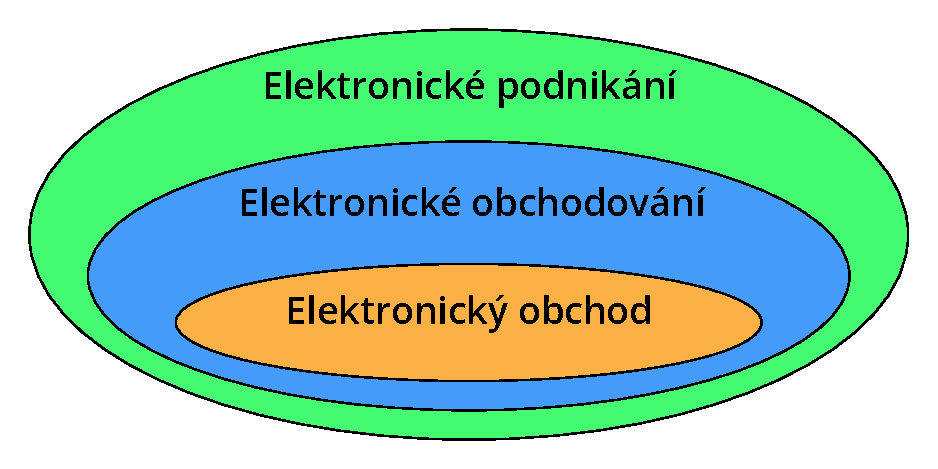
\includegraphics[width=\textwidth]{e-commerce.pdf}
\caption{Vztah elektronického podnikání, obchodování a podnikání}
\label{e-commerce}
\end{figure}

Zcela zásadní výhodou elektronického obchodu oproti návštěvě obchodu kamenného
je možnost vytvoření objednávky z pohodlí domova a její následné doručení zásilkovou 
službou. Tento přístup především šetří čas strávený cestou do obchodu a čas strávený 
v~obchodě. Například v segmentu nákupu potravin může být výhodou to, že je takový 
nákup hygieničtější a zboží bude doručeno v lepším stavu díky uzpůsobeným vozům dopravců.
Výhody ale vznikají i pro provozovatele -- nemusí zřizovat prodejnu včetně jejího vybavení a 
zaměstnance, mohou efektivněji navrhnout sklad, nebo dokonce využít automatizace 
při kompletaci objednaného zboží.

\subsection*{Plnotextové vyhledávání}

Plnotextové vyhledávání (full-text search), je způsob vyhledávání v textových datech, 
kdy se vyhledává uživatelem formulovaný dotaz v invertovaném souboru (někdy také 
indexovém souboru nebo invertovaném indexu), tedy v souboru obsahující výrazy, 
podle nichž je daný záznam vyhledatelný \cite[strana~15]{strossa}. 
Proces, kterým vzniká indexový soubor se nazývá indexace. Tato problematika je podrobněji
popisována v druhé kapitole.

\section{Vysvětlení problému, který je řešen}

Plnotextové vyhledávání je rychlým prostředkem nalezení konkrétního produktu
v elektronickém obchodě. Typicky je využito zákazníky, kteří jsou na webu
s konkrétní potřebou a jsou schopni formulovat výraz, podle kterého produkt
hledají. Může jít o název tybu produktu, jeho značku, variantu nebo kategorii.
Pro takového uživatele je procházení webu procházením kategorií zdlouhavé
a právě plnotextové vyhledávání mu může zásadně zrychlit cestu k nalezení 
hledaného produktu.

Důležitost plnotextového vyhledávání navíc roste s rostoucím počtem produktů a kategorií, 
v kterých je složité se orientovat. Uživatel tak může vyhledávání využít už pro 
nalezení kategorie, která se nachází v dlouhém a nepřehledném menu.

\begin{figure}[h]
\center
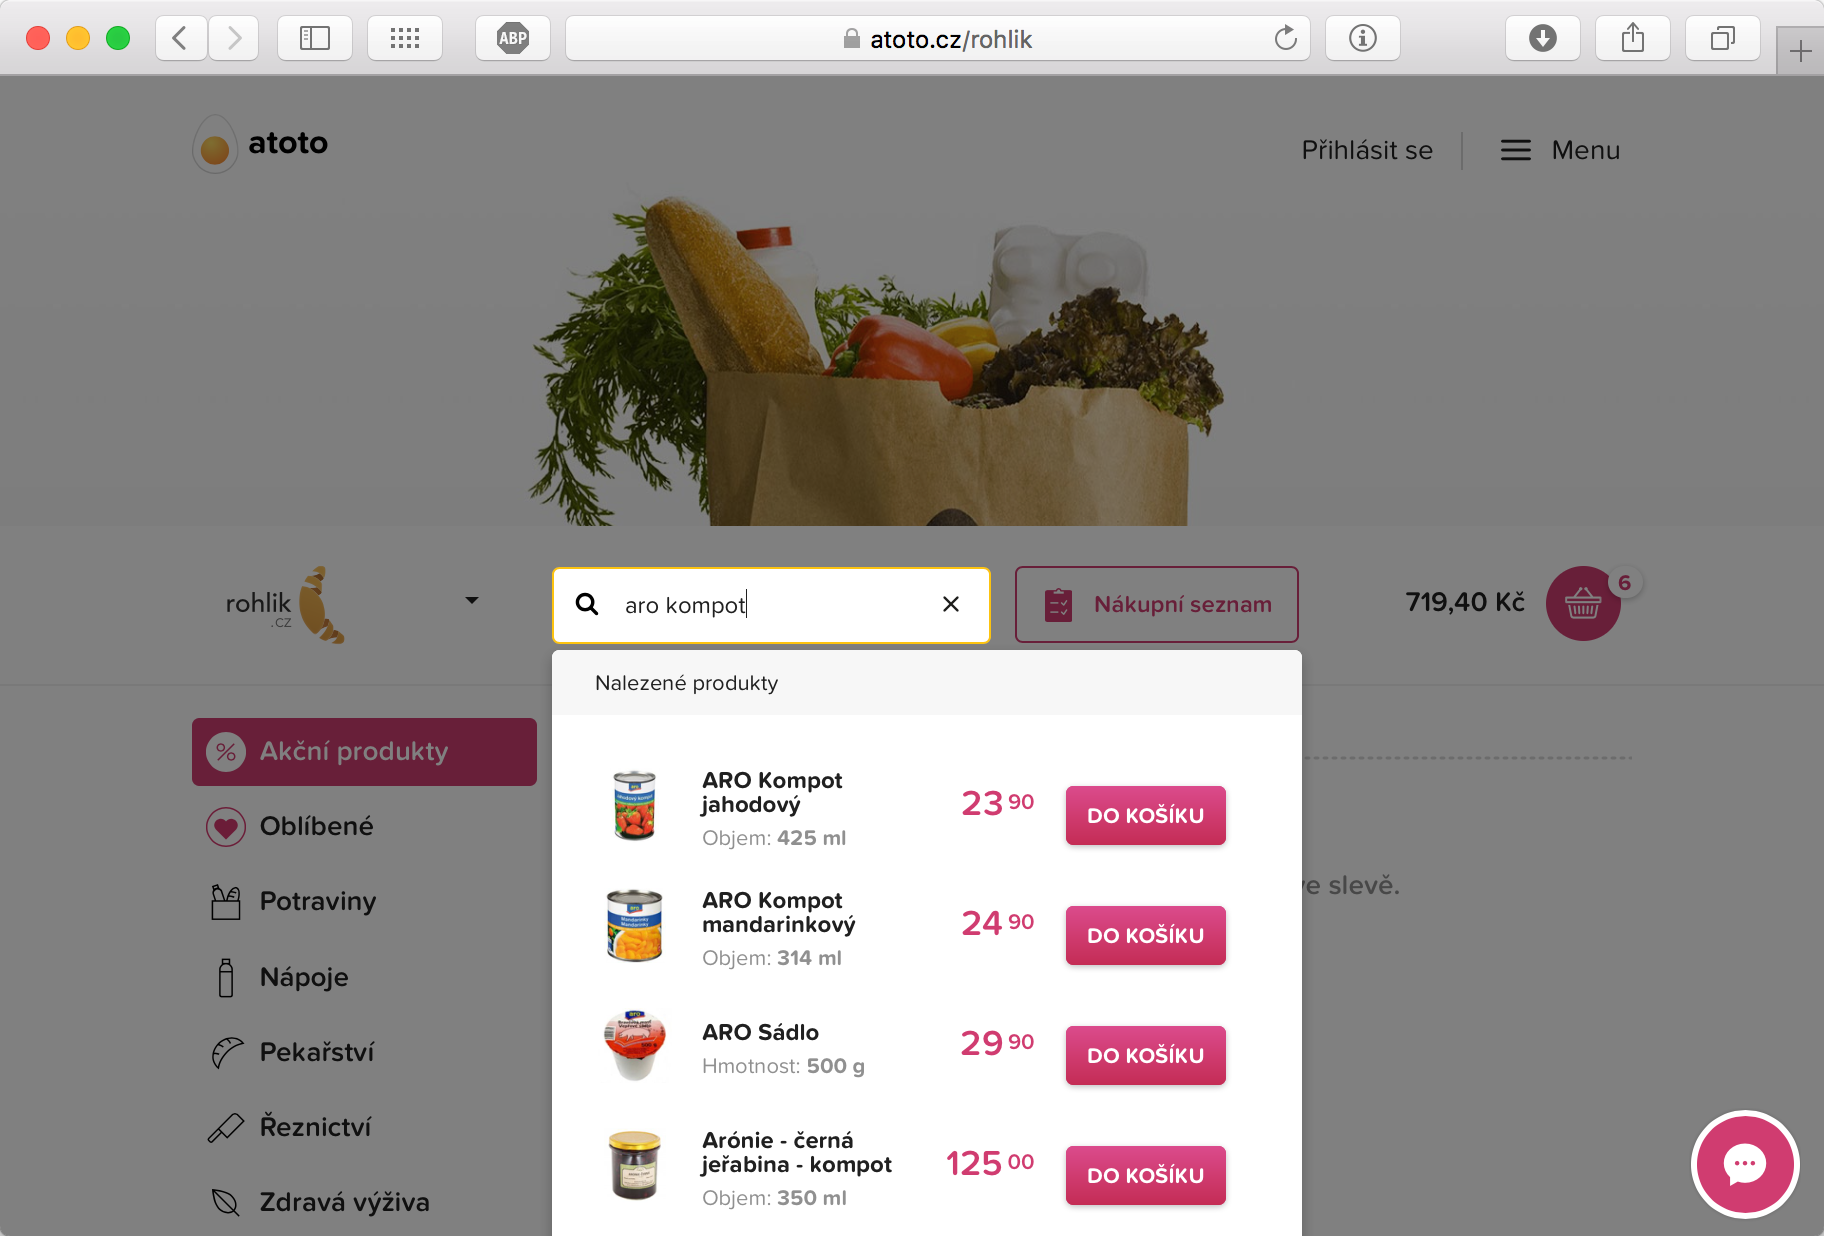
\includegraphics[width=\textwidth]{atoto-vyhledavani.png}
\caption{Ukázka plnotextového vyhledávání v elektronickém obchodu}
\label{atoto-vyhledavani}
\end{figure}

Implementace plnotextového vyhledávání však není triviální záležitostí. Vstup uživatele
je v přirozeném jazyce, takže je třeba jej odpovídajícím způsobem zpracovat, 
aby bylo vůbec vyhledávání na webu použitelné. Studium této problematiky
může být zdlouhavé a v konečném důsledku drahé. Pokud bude k dispozici hotové řešení, 
které bude snadno nasaditelné na elektronický obchod a bude umožňovat jednoduché 
uzpůsobení potřebám konkrétního webu, bude to výrazná úspora jak času, tak peněz
provozovatele obchodu.

\section{Specifika elektronického obchodování}

V prostředí elektronického obchodování existují jisté vzorce které se opakují a odlišují
toto prostředí od ostatních. Vyhledávají se zpravidla produkty (případně služby), které jsou
zařazeny do určitých kategorií a disponují atributy jako cena, název, kód, popis, url, obrázek, 
dostupnost a dalšími parametry, které bývají číselné (hmotnost, objem) nebo výčtové (barva, značka). 

Z toho vyplývá co a podle čeho se bude vyhledávat. Produkty mívají jednoznačné identifikátory, 
které jsou navíc standardizovány (EAN, ISBN). Pomocí těchto kódu je možné vyhledat produkty
napříč elektronickými obchody nebo je párovat v cenových srovnávačích. Pro vyhledávání
je dále důležitý název produktu, případně jeho varianty, která upřesňuje konkrétní
verzi produktu. Méně častěji je nutné vyhledávat v popisu produktu, kde bývá uveden
jak slovní popis, tak výpis parametrů. 

U produktů dále bývá evidována cena, která může být interně uložena v kombinaci s marží.
Obchody operující se zlevněným zbožím pak mívají uvedenou cenu jak před slevou, tak po této
slevě, aby zákazník viděl, kolikaprocentní sleva je na produktu. I samotná cena produktu
(případně marže prodejce) může hrát svou roli ve vyhledávání.

\section{Definice požadavků na vyhledávání}

Požadavky na samotné vyhledávání jsou ovlivněny prostředím, ve kterém vyhledávání
probíhá a uživateli, kteří vyhledávání využívají. Primárně by mělo být možné
nalézt daný produkt podle jeho názvu, nebo části názvu. To samé platí pro 
kód produktu. Produkt by měl být ale vyhledatelný i podle dalších atributů, 
jako je název kategorie nebo název značky výrobce. Někdy dokonce uživatel nemusí
vyhledávat konkrétní produkt, ale jen produkty dané značky nebo kategorie, což by
měl systém také umět rozpoznat.

Podoba vyhledávaných výrazů bude zadávána zákazníky v přirozeném jazyce, s čímž by si mělo
vyhledávání také poradit. Konkrétně jde o tvarosloví, kdy může uživatel zadat výraz
například v jiném pádu, než je uvedeno v názvu produktu. Dále jde o vyrovnání se
s~chybami, které mohou vzniknout při formulaci vyhledávaného výrazu -- překlepy nebo
pravopisné chyby. V neposlední řadě jde také o vztah slova k jeho významu, kdy může
jedno slovo mít více významů (homonymum) nebo naopak více slov může odpovídat jednomu výrazu
(synonymum).

Další problematikou při zadávání hledaného výrazu uživatelem, je poskytování relevantních výsledků
už ve chvíli, kdy uživatel formuluje dotaz, tedy jej teprve píše. V takovém případě je třeba
odhadnout, který výraz chce napsat a tuto informaci využít při zobrazení odpovídajících
výsledků.

Ve chvíli, kdy systém zná produkty, které odpovídají hledanému výrazu by měl
výsledky poskytovat ve vhodném pořadí, měl by tedy pracovat s relevancí výsledků vzhledem 
k~zadanému výrazu. Toto může být velmi obtížné, protože každý uživatel má zájem o jiné
produkty a tak pro něj mohou být ro jeden výraz relevantní jiné produkty, než pro někoho
jiného. Dále do tohoto pořadí můžou vstupovat požadavky provozovatele elektronického obchodu
v případě, kdy má specifické požadavky na zboží, které chce nabízet přednostně. Důvodů
pro takové chování může být více, může souviset s marží konkrétních produktů, 
nebo s filozofií samotného obchodu.

\section{Technické požadavky na aplikaci}

Na aplikaci je kladeno několik technických požadavků. Nejedná se o funkční požadavky, nýbrž
o požadavky související s použitelností, výkonností, spolehlivostí a podporou. Naplnění těchto
požadavků zajistí následný bezproblémový chod aplikace a uspokojení potřeb zákazníka.

Prvním technickým požadavkem na aplikaci je její rychlost. Ta je důležitá pro spokojenost
koncového zákazníka, který provádí vyhledávání. Všechny části aplikace nejsou z hlediska rychlosti
tak kritické, jedná se primárně o samotné vyhledávání. Akceptovatelná rychlost uživatelského rozhraní 
v tomto případě je 100 ms \cite{amazon-100ms}, v ideálním případě do 50 ms \cite{stackshare-algolia}. 
Pro naplnění tohoto požadavku je třeba, aby byla rychlost odezvy API co nejnižší.
Rychlost by dále nemělo výrazně ovlivňovat množství současných požadavků. 
Aplikace by měla být navržena tak, aby ji bylo možné snadno škálovat při zvyšující se zátěži.

Dalším požadavkem je formát samotného API. Bude třeba použít takový formát, který bude
co nejsnadněji implementovaný v používaných webových technologiích pokud možno bez instalace
jakýchkoli rozšíření. To je důležité pro rychlé nasazení aplikace do provozu a odbourání
možných vstupních bariér při rozhodování o využití nástroje. Pro načtení produktů
z elektronických obchodů by bylo ideální využít stávajících exportů pro jiné systémy, 
kterými by obchody mohly implementovat. Pokud by nic takového neexistovalo, můsí být vytvoření
export produktů pro provozovatele elektronického obchodu co nejsnažší.

Posledním technickým požadavkem je dokukemantace samotného API. Dokumentace musí být
dobře pochopitelná, tedy psaná přehledně, ideálně s konkrétními ukázkami použití.
Výhodou je také možnost vyzkoušet si práci s API vůči testovacímu prostředí, 
kde nebude riziko vzniku chyb na produkčních datech.

\section{Popis oborů, kterých se práce dotýká}

Samotné řešení problematiky vyhledávání je výrazně interdisciplinární obor. Je nutné
mít značné povědomí o získávání informací, počítačovém zpracování přirozeného jazyka, 
což souvisí jak s počítačovou lingvistikou, tak úzce s teorií formálních jazyků a překladačů.
Existuje také vztah mezi lingvistikou a logikou, jakožto vědě o myšlení, která se odehrává 
v kategoriích lidského jazyka. Podobný vztah lze nalézt také s umělou inteligencí, 
vzhledem k tomu, že používání přirozeného jazyka je inteligentní činností.
Díky tomu, že probíhá ukládání dat, je důležitá znalost teorie datových modelů.
Vzhledem k množství ukládaných dat se také můžeme dotýkat oboru Big Data.
V neposlední řadě je třeba porozumnět potřebám potenciálních uživatelů, tedy mít
určitou znalost podnikání a obchodování.

\section{Stávající možnosti implementace vyhledávání}

Na trhu existuje několik služeb, které umožňují implementaci plnotextového vyhledávání.
Ty se však liší funkčností, obtížností implementace i cenou. Níže popisuji nejvýznamější 
z nich zejména vzhledem k požadavkům na aplikaci.

\subsection{Využití relační databáze}

První možností, jak vyhledávání implementovat je využití stávající databáze, 
kterou elektronický obchod disponuje. Ať už se jedná o open source (MySQL, Postgres)
nebo konerční (SQL Server, Oracle) databázi, možnosti plnotextového vyhledávání
jsou zde omezené. Výhodou je to, že jsou data stále v jednom úložišti, není třeba
řešit správu (instalaci, konfiguraci nebo zálohování) dalšího nástroje. Ani vývojáři 
se nemusí učit nic nového, pouze využijí stávající databázi. Vyhledávání zde probíhá
v nejjednodušší formě pomocí operátoru \verb|LIKE|. Některé databázové systémy
mají disponují pokročilejšími funkcemi, kterými lze vyhledávání zlepšit \cite{postgres}.

\subsection{Elasticsearch, Solr, Sphinx}

Využitím nástrojů přímo určených pro implementaci plnotextového vyhledávání lze 
dosáhnout nejlepších výsledků, ať už se jedná o Elasticseacrch či Apache Solr využívající
Apache Lucene \cite{lucene}, nebo Sphinx. Jde o typický krok v okamžiku, kdy
přestává funkčnost relační databáze pro potřeby vyhledávání dostačovat. Tyto nástroje
umožňují pokročilé nastavení indexace a zároveň jsou dostatečně rychlé, aby byly
schopny provádět vyhledávání v řádu milisekund. Zřejmou nevýhodou tohoto řešení
je nutnost znalosti dalšího nástroje, jeho správa a řešení synchronizace se 
stávající databází.

\subsection{Algolia}

Algolia je pokročilý nástroj umožňující imlementaci plnotextového vyhledávání \cite{algolia}. 
Zaměřuje se na poskytování kvalitních výsledků v co nejkratším možném čase (v řádu milisekund). 
Snaží se usnadnit práci programátorům tím, že nabízí řadu připravených integrací 
pro konkrétní programovací jazyky a frameworky. Kromě výsledků vyhledávání umožňuje 
faceting, tedy dodání dat pro tvorbu filtrů, podporuje řadu jazyků nebo vyhledávání 
podle geografické lokality. V neposlední řadě je k dispozici dashboard zobrazující 
stav systému a statistiky vyhledávání.

Pokud si zákazník vystačí s 10 000 vyhledatelnými produkty, může nástroj Algolia používat
zdarma, pouze je povinnen uvést ve výsledcích vyhledávání logo firmy. Placené verze 
začínají na 59 dolarech za měsíc za 100 000 produktů.

\subsection{Swiftype Site Search}

Swiftype Site Search je nástroj podobný nástroji Algolia, zaměřuje se však více na 
uživatelské rohraní a celkově na snadnost použití \cite{swiftype}. Mezi jeho hlavní
funkce patří vyhledávání v okamžiku formulace hledaného výrazu, možnost filtrace
výsledků, dodatečná úprava pořadí výsledků ručním zásahem na úrovni konkrétních 
výsledků, nebo na základě některého z atributů produktu. V nesposlední řadě je také
k dispozici přehledná analytika proběhlého vyhledávání. Cena za provoz služby
začíná na 299 USD měsíčně.

\subsection{AWS CloudSearch}

Firma Amazon poskytuje v rámci svého cloudu službu CloudSearch \cite{cloud-search}.
Jejími přednostmi jsou především vysoká výkonnost a škálovatelnost. Velkou vstupní
bariérou je však její počáteční složitost. Uživatel musí nejprve proniknout do 
některých základních konceptů Amazon Web Services, až poté může začít pracovat
se samotným vyhledáváním. Co se funkčnosti týče, nabízí služba podporu 34 jazyků, 
možnost nastavení váhy jednotlivých atributů, nebo doplňování texu během psaní.
Cena záleží na využití výpočetní kapacity, její určení je tedy složitější.

\subsection{Google Custom Search Engine}

Google Custom Search Engine \cite{gse} se nejvíc odlišuje od ostatních služeb. 
Vyhledávání je plně řízeno algoritmem společnosti Google a také výsledky vyhledávání
vypadají obdobně, jako výsledky vyhledávání na www.google.com. 
Odlišné je i samotné napojení na službu -- výsledky vyhledávání jsou na web
vloženy jako samostatná stránka, na které je vidět logo společnosti Google.
Základní varianta je však zdarma, je to tedy levná cesta, jak rychle zprovoznit
vyhledávání na webu. Pokročilejší varianta umožňující konfiguraci stojí 100 USD ročně.

%\subsection{Porovnání, odůvodnění vytváření nového nástroje}
%
%\begin{figure}[h]
%\center
%
\includegraphics[width=\textwidth]{todo.pdf}
%\caption{Tabulka s porovnáním nástrojů pro vyhledávání}
%\end{figure}
%
% TODO: okomentování tabulky, vysvětlení, proč se vytváří nový nástroj


%%%%%%%%%%%%%%%%%%%%%%%%%%%%
\chapter{Plnotextové vyhledávání}

Tato kapitola popisuje problematiku textového vyhledávání a poukazuje tak na konkrétní
problémy, které je při vyhledávání nutno řešit. Problematika je rozebírána v kontextu
elektronického obchodování, jsou tedy uváděny pouze principy aplikovatelné v tomto
oboru.

Vyhledávání je proces sestávající jednak z ukládání dokumentů určených k~vyhledávání
a dále z provedení vyhledávání uživatelem. Obecné schéma vyhledávání vypadá následovně:

\begin{figure}[h]
\center
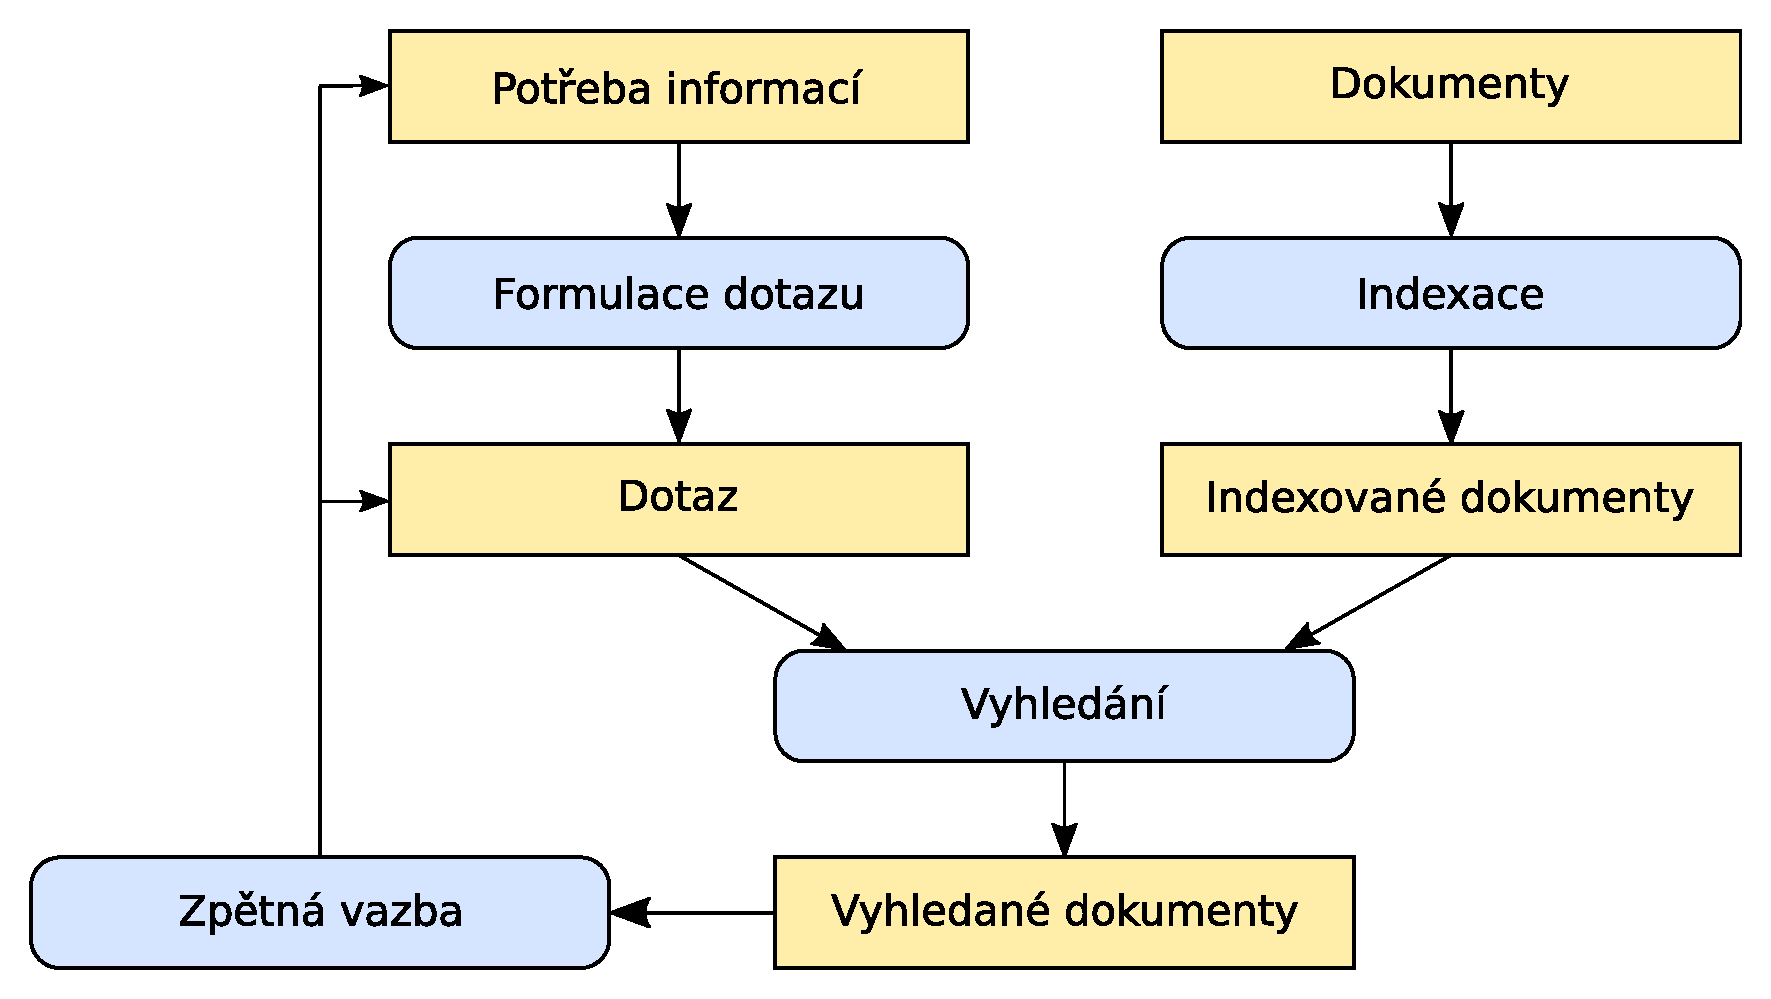
\includegraphics[width=\textwidth]{schema-vyhledavani.pdf}
\caption{Proces vyhledávání}
\label{schema-vyhledavani}
\end{figure}

Ukládání dokumentů probíhá tak, že se upraví pro potřeby vyhledávání a uloží 
do indexu, přičemž celý tento proces se označuje jako indexace. Ve chvíli, kdy jsou
dokumenty připraveny k vyhledávání, může uživatel mající potřebu v těchto dokumentech 
vyhledávat (získávat z nich informace) formulovat dotaz, kterým chce získat odpovídající
dokumenty. Z něj je vytvořen dotaz, podle nějž bude vyhledávání provedeno. Následně
jsou uživateli dodány dokumenty vyhovující dotazu, ten pak může dotaz na základě
získaných dokumentů a pochopení způsobu vyhledávání dotaz upravit.

\section{Analýza dat, v kterých bude vyhledáváno}

Nejprve je třeba prozkoumat data, ve kterých bude vyhledávání prováděno. Vycházím
ze~skutečnosti, že naprostá většina elektronických obchodů své zvoží nabízí také 
prostřednictvím srovnávačů zboží, přičemž v počtu návštěv a tedy celkovém provozu 
v~rámci českého internetu jsou nejdůležitější Heureka.cz a Zboží.cz \cite{netmonitor}. 

Data pro tyto srovnávače musí být dodávána prostředníctvím XML feedu, který odpovídá 
specifikaci jednotlivých systémů. Při porovnání obou specifikací lze nalézt 
jistou podobnost v požadovaných údajích. Samotný XML feed obsahuje
produkty obchodu, přičemž u každého produktu je možné uvést několik atributů, z~nichž
některé jsou povinné. Konkrétně v případě Zboží.cz musí mít každý produkt uveden název, 
popis, URL, cenu a dostupnost. Dále lze využít volitelných parametrů jako název kategorie, 
název značky a výrobce, EAN, ISBN, produktový kód výrobce, případně další doplňkové
informace a parametry \cite{xml-zbozi}. V případě Heuréka.cz je podstatný název
obsahující případně výrobce a produktové číslo či kód, název kategorie, dostupnost a
cena dopravy. Informace o produktu mohou dále obsahovat popis, EAN, kód produktu
nebo soupis parametrů \cite{xml-heureka}. Minimální XML soubor s jedním produktem 
ve formátu Heuréka by vypadal následovně:

\begin{minted}{xml}
<?xml version="1.0" encoding="UTF-8"?>
<SHOP>
 <SHOPITEM>
  <ITEM_ID>40272131</ITEM_ID>
  <PRODUCT>
   Matrace MYRBACKA - Latexová matrace, střední tvrdost, bílá
  </PRODUCT>
  <PRODUCTNAME>Matrace MYRBACKA</PRODUCTNAME>
  <DESCRIPTION>
   <![CDATA[Latex vám umožní lépe odpočívat a to tak, že sleduje
    kontury vašeho těla, uvolňuje tlak a poskytuje precizní podporu.
     - Potah: 64% polyester, 36% bavlna
     - Vnitřní látka: Netkaný polypropylen, 100% jehněčí vlna
     - Komfortní materiál: syntetický latex, polyuretanová pěna]]>
  </DESCRIPTION>
  <URL>http://ikea.com/cz/cs/catalog/products/40272131</URL>
  <IMGURL>http://ikea.com/cz/cs/images/products/40272131.JPG</IMGURL>
  <PRICE>9087</PRICE>
  <PRICE_VAT>10990</PRICE_VAT>
  <CATEGORYTEXT>Dům a nábytek | Nábytek | Matrace</CATEGORYTEXT>
  <MANUFACTURER>IKEA</MANUFACTURER>
 </SHOPITEM>
</SHOP>
\end{minted}

Na základě znalosti struktury feedů lze zjistit, že při využití stávajících XML exportů
internetových obchodů bude každý produkt obsahovat název, popis, URL, cenu, dostupnost
a název kategorie, přičemž pravděpodobně bude k dispozici řada dalších atributů, 
dle použetého formátu feedu a dle pečlivosti provozovatele obchodu.

\section{Automatické indexování textů}

Indexování je proces, kdy jsou ukládány textové dokumenty určené k vyhledání.
Ukládány jsou použe výrazy, podle nichž by měl být ukládaný dokument vyhledatelný. 
Místo, kam jsou tyto výrazy ukládány se nazývá index. Jedná se vlastně o klíče, 
podle kterých bude bude možné rychle hledaný záznam nalézt. To je důležité z hlediska
rychlosti vyhledávání -- není možné všechny uložené záznamy procházet a analyzovat
až ve chvíli vyhledávání. 

Při indexování je třeba analyzovat každý výraz, který by měl být uložen do indexu.
V prvé řadě je třeba rozhodnout, zda je třeba jej do indexu ukládat, je tedy 
třeba řešit významnost jednotlivých výrazů v textu. Pokud daný
výraz není pro vyhledávání užitečný, nemá smysl jej ukládat. Dalším problémem je 
tvarosloví, tedy to, že slova mohou měnit tvar (jedná se například o skloňování 
podstatných jmen), stále se přitom jedná o jedno slovo. V neposlední řadě je také 
třeba zohlednit význam slov v daném oboru, kdy mohou stejná slova vyjadřovat jiné věci 
(homonymie -- například myš ve smyslu počítačového příslušenství a myš jako zvíře), 
nebo může být jeden význam vyjádřen různými slovy (synonymie -- lednička i chladnička 
označuje totéž). Konečně je také třeba brát v úvahu další vztahy mezi slovy, 
jako nadřazenost a podřazenost. Například banán a ovoce mohou označovat totéž, 
přičemž ovoce to činí v širším slova smyslu, toto označení lze použít i pro jiné 
ovoce, například jablko.

\section{Specifika českého jazyka}

Vzhledem k tomu, že je vyhledávání vytvářeno pro čecké internetové obchody, 
bude veškeré vyhledávání probíhat v českém jazyce, proto nyní popíšu jeho specifika.
Český jazyk pracuje se slovy odlišně než jiné jazyky. Dále dochází k drobným
odchylkám i v rámci českého jazyka na základě geografické oblasti (nářečí)
nebo na základě zaměření dané skupiny lidí (hantýrka). Dále se můžeme zabývat
grafickou podobou jazyka (morfologií) nebo jeho zvukovou podobou (fonetikou).
Vzhledem k tomu, že vyhledávání probíhá na textové bázi, zabývám se dále právě 
grafickou podobou jazyka.

Slova jsou v českém jazyce řazena do slovních druhů, kterých je celkem deset.
Slovní druh pomáhá určit chování slova -- slova stejného slovního druhu se ohýbají
a vyskytují v textu podle podobných pravidel. Slovní druhy lze dělit podle
toho, zda jsou ohebné (tedy zda se jejich tvar může měnit) a neohebné.
Neohebné slovní druhy jsou zpravidla používány ve větě společně s obehnými, 
protože samy o sobě nenesou informační hodnotu. Naopak ohebné slovní druhy
samy o sobě nesou informační hodnotu, jsou proto vhodnými kandidáty pro
to, aby se podle nich vyhledávalo. Výjimkou jsou zde zájmena, která nesou 
informaci nepřímo.

\begin{figure}[h]
\center
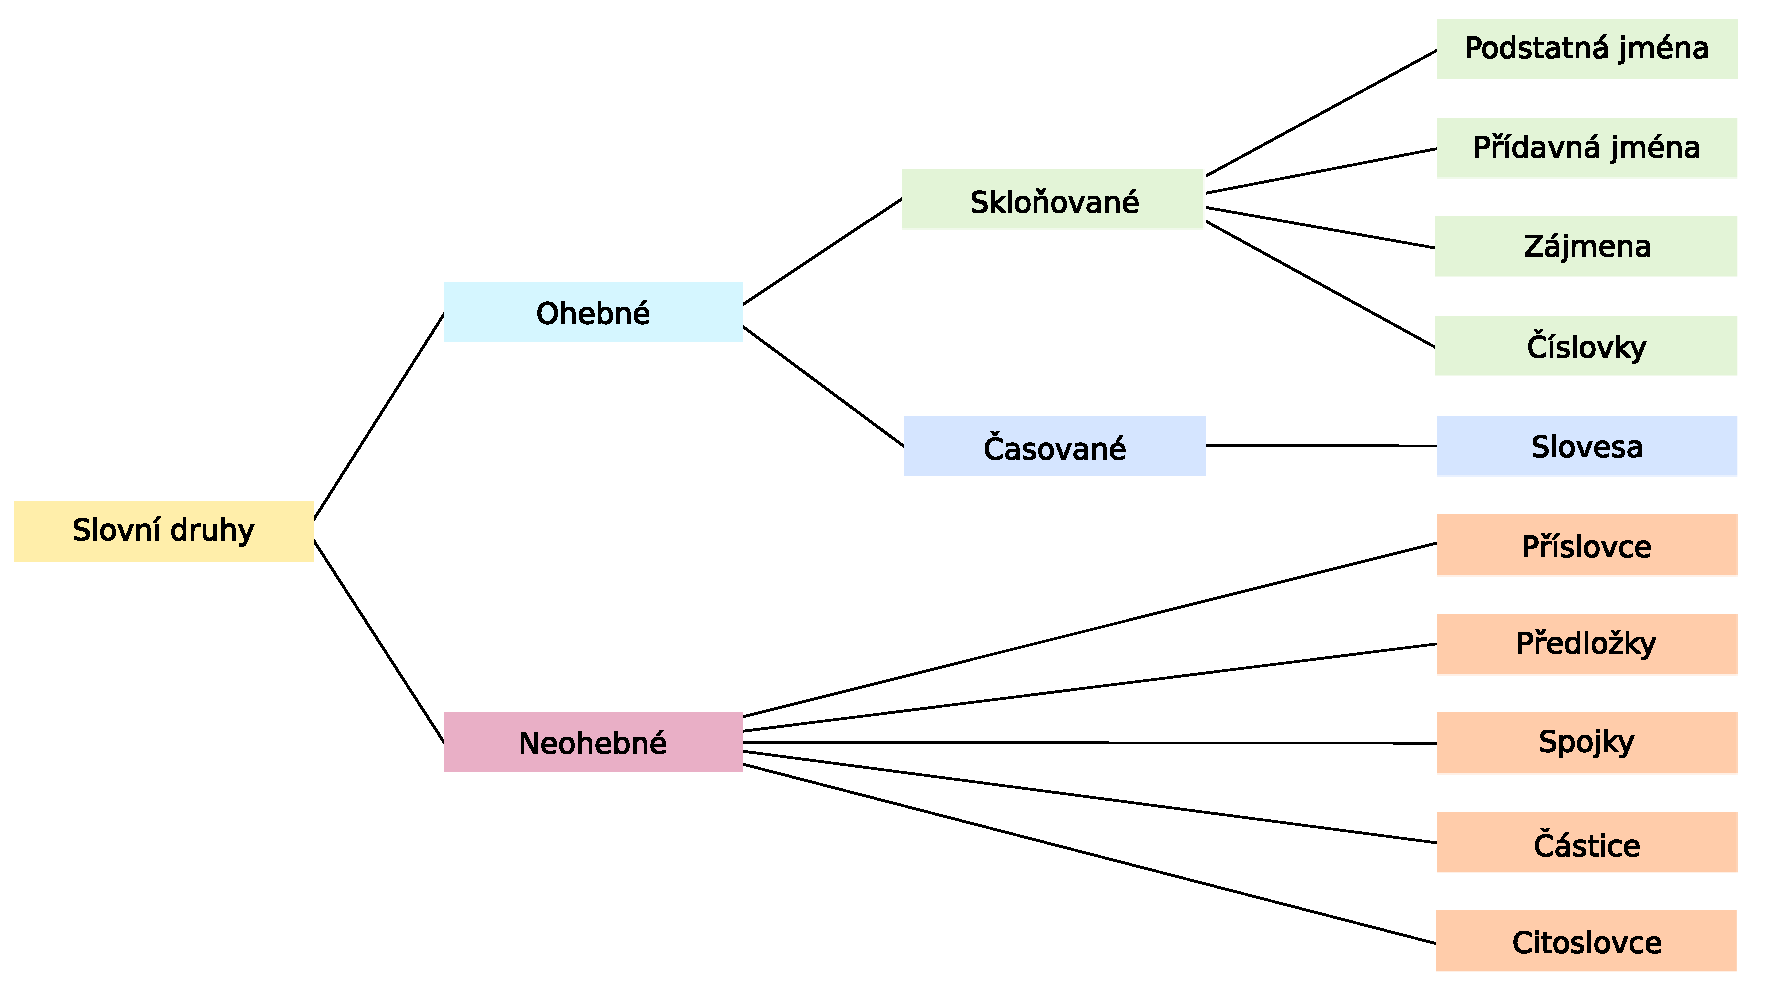
\includegraphics[width=\textwidth]{slovni-druhy.pdf}
\caption{Dělění slovních druhů dle jejich ohebnosti}
\label{slovni-druhy}
\end{figure}

V rámci ohebnosti lze rozlišovat jakým způsobem jsou ohýbána. Slovesa mohou být
časována, příslovce mohou být stupňována, podstatná jména, přídavná jména, zájmena
a číslovky mohou být skloňována. Dále v češtině rozlišujeme tři jmenné rody
(mužský, ženský a střední) a dvě čísla (jednotné a množné). U sloves dále 
rozlišujeme jejich vid.

\section{Problematika tvarosloví}

První problém související s zpracováním přirozeného jazyka je vypořádání se s tvaroslovím
(morfologií). Jednotlivá slova se v českých textech objevují v různých slovních tvarech, 
málokdy jsou všechna slova v základním tvaru. Například jeden produkt může mít název
"Alex Čistič na laminát s pomerančovým olejem" i "Alex čistič na laminát pomerančový olej".
V obou případech je uveden pomeranč, jen v různém tvaru. Při vyhledávání však
chceme docílit toho, aby byla obě slova vyhledatelná shodně, ať už bude slovo pomeranč
zadáno v kterémkoli pádě. Typické řešení je vřazení modulu do procesu indexace dokumentů nebo 
dotazů, který sjednocuje podobu zadaných slov.

\subsection{Základní pojmy tvarosloví}

Nejprve vysvětlím základní pojmy rozebíraného oboru, jejichž znalost je nutná k pochopení 
následujícího textu.

\subsubsection*{Morfém}

Morfém je minimální funkční jednotka s vlastním významem. Jde o základní jednotku vědy, 
která se zabývá tvorbou slov, tedy morfologie.

\subsubsection*{Lexém}

Lexém je základní stavební jednotka slovníku, znaková jednotka vyjadřující pojem nesoucí
význam. Je to základní jednotka vědy zabývající se slovní zásobou -- lexikologie. Ta je stejně 
jako morfologie odvětvím lingvistiky. Každý lexém je pak možné dále dělit na koncovku, 
kmen, kořen, prefix a sufix.

\subsubsection*{Foném}

Foném je hláska umožňující rozlišit význam. Obory, pod které spadá, se zabývají zvukovou
stránkou jazyka a nazývají se fonetika a fonologie.

\subsubsection*{Flexe}

Flexe neboli ohýbání popisuje změnu slov vzniklou při skloňování, časování nebo ohýbání.
Jde o grafickou změnu lexému pro vyjádření odpovídajícího pádu, rodu a dalších gramtických
kategorií.

\subsection{Operátor pravostranného rozšíření}

Nejjednodušším řešením problematiky ohýbání slov je operátor pravostranného rozšíření.
Mějme slovo svíčka, které se při skloňování v jednotném čísle mění na svíčky, svíčce, 
svíčku, svíčko, svíčce, svíčkou. V tomto příkladu lze vypozorovat, že se mění
pouze konec slova, zatímco levá část \textbf{svíčk-} zůstává stejná. Tento přístup bude 
sice poměrně úspěšný, nicméně se nevyhneme případům, kdy bude mít více slov stejný
základní tvar. Mohli bychom tak při vyhledání výrazu \textbf{svíčk} obdržet dokumenty
obsahující slovo \textbf{svíčková}.

Vzhledem k jednoduchosti a zároveň poměrně vysoké úspěšnosti bývá tento přístup
často využíván jako jedna z prvních implementací plnotextového vyhledávání přímo
v relační databázi pomocí operátoru \verb|LIKE|. Konkrétně vyhledávání v jazyce SQL
výše diskutovaného výrazu by bylo provedeno jako \verb|LIKE 'pomeranč%'|.

Kromě problému s možným shodným základem pro různá slova je další komplikací při 
použití této metody skutečnost, že při ohýbání slov nedochází pouze ke změně koncovek, 
ale často se mění také některá písmena základu slova. Uvažujme slovo \textbf{kůň}, které
má v~druhém pádu podobu \textbf{koně}. Pro tento případ by bylo možné rozšířit možnost 
pravostranného rozšíření o nahrazení pouze jednoho znaku. Pokud bychom tak měli 
pro nahrazení více písmen využít znak \textbf{*} a pro nahrazení právě jednoho písmene 
znak \textbf{?}, byl by základní tvar tohoto slova \textbf{k?ň*}. To je ale problém, protože 
takový výraz odpovídá například i slovu \textbf{kaňka}.

\subsection{Derivátor slovních tvarů}

Derivátor slovních tvarů je nástroj, který namísto daného slova vygeneruje 
všechny jeho gramatické tvary, případně jeho použitelné odvozeniny. 
Ty jsou následně používány jako jejich logická disjunkce. Například místo 
slova \verb|svíčka| by se použilo:

\begin{figure}[thp]
\centering 
\begin{minipage}{0.7\textwidth}
\begin{minted}{bash}
(svíčky OR svíčce OR svíčku OR svíčko OR svíčkou 
  OR svíček OR svíčkám OR svíčkami OR svíčkách)
\end{minted}
\end{minipage}
\end{figure}

Takový systém musí obsahovat co nejpřesnější sadu pravidel, jak vytvářet
veškeré tvary zadaného slova. Dale je třeba k expandovanému slovu zadat
jeho veškeré informace, aby mohlo být vybráno správné pravidlo.

\subsection{Stematizace}

Stematizace je proces, kdy je slovo převáděno na jeho kmen (stem). Toho je docíleno
odstraněním předpon, přípon a koncovek. Její použití je vhodné pro jazyky, 
které mění slova jen tímto způsobem (např. Angličtina). Pro češtinu je však stematizace
hůře aplikovatelná, protože se slova ohýbají podle složitějších pravidel, ne jen
změnou předpon, přípon nebo koncovek. Stematizaci tedy využít při hledání základního
tvaru slova v českém jazyce, je ale nutné ji rozšířit o další procesy, které jsou 
popisovány dále.

\subsection{Lematizace}

Lematizátor je nástroj, který převádí slovo na jeho základní gramatický tvar, tzv. lemma.
Základním gramatickým tvarem se roumí první pád jednotného čísla u podstatných jmen nebo infnitiv 
u sloves. Celý proces se nazývá lematizace a kromě převodu na základní tvar může lematizátor
disponovat doplňkovou funkcí, kdy pro daný tvar poskytne i jeho tvaru, například 
slovní druh, pád nebo číslo. Lematizátor pracuje v podstatě opačně ve srovnání s derivátorem. 
Lematizace zároveň není totéž co stematizace, které předpokládá, že dochází 
jen k přidávání předpon a přípon. Lematizátor jej vpodstatě rozšiřuje, odstranění
předpon nebo přípon však může být jednou jeho z činností. Především ale počítá s~tím, 
že se koncovky nebo kmeny slov mohou měnit, což je důležité pro češtinu.
Dalším rozdílem je výsledek daného procesu -- po stematizaci může vzniknout díky ořezání
předpon a přípon neexistující slovo, výstupem lematizace je však vždy slovo existující.

Algoritmů pro implementaci lematizátoru je více, triviálním řešením může být použití
slovníku, který obsahuje veškerou slovní zásobu daného jazyka a všechny tvary těchto
slov. V něm je pak nalezeno slovo v daném tvaru a k němu odpovídající základní tvar.
Výhodou takového přístupu je přesnost lematizace, pokud je již daný tvar slova znám, 
je triviální najít přesný základní tvar. Jediný problém může způsobit duplicita daného 
slova, kdy se musí lematizátor rozhodnout, na kteroý základní tvar jej upraví. Nevýhodou
je poté nutnost vytvoření takového slovníku, kdy je třeba popsat veškerou slovní zásobu.

Další možností je algoritmická lematizace, kdy jsou definována pravidla, podle kterých jsou
slova ohýbána a ta jsou používána pro hledání základního tvaru. Využití takového přístupu
znamená daleko menší soubor pravidel, podle kterých je lematizace prováděna ve srvnání 
s~kompletním slovníkem slovní zásoby. Je tedy rychlejší takový lematizátor vybudovat
od počátku a ve srovnání s použitím slovníku je velká šance, že bude správně zpracováno
neznámé slovo. Pokud chybí ve slovníku, nelze rozhodnout, jak lema vytvořit. Pokud
však budeme mít definovánu jen sadu pravidel, spíše bue lematizace provedena úspěšně.
Zřejmou nevýhodou ve srovnání s využitím slovnku je kvalita takové lematizace. 
Čeština je dosti nepravidelná a existuje mnoho výjimek, které se při ohýbání slov vyskytují.

Konečně lze také pro lematizaci využít stochastických metod, respektive metod strojového
učení. Ručně se vytvoří trénovací data, která se následně použijí pro vytvoření modelu.
Na základě tohoto modelu lze provádět samotnou lematizaci, přičemž použitelných metod 
strojového učení je celá řada. Každý z zde uvedených přístupů má své výhody a nevýhody, 
nejlepších výsledků však bude možné dosáhnout jejich kombinací a vhodným nastavením.

\section{Problematika významnosti}

Další problém, který je třeba řešit je významnost výrazů, podle nichž je vyhledáváno.
Ne všechna slova jsou pro vyhledávání využitelná, protože nenesou žádnou užitečnou 
hodnotu, nebo jsou tak častá, že je jejich využití degradováno. 

Zároveň však ne všechna slova charakterizují daný dokument stejnou mírou. Nelze se tedy 
jen rozhodovat, zda dané slovo ukládat do invertovaného indexu, je také třeba pamatovat
na rozdílnou informační hodnotu slov vůči dokumentům -- ať už se jedná o indexovaný
dokument, nebo o celou jejich sadu.

\subsection{Negativní slovník}

Negativní slovník, někdy označovaný také jako stop-slovník nebo slovník stop-slov, 
je datová struktura obsahující slova, která jsou v daném případě považována za bezvýznamná
z pohledu vyhledávání. Bývají to slova určitých slovních druhů, nebo obecně slova, která 
nenesou žádný význam. Obvykle jde o předložky, spojky nebo zájmena. Někdy také může jít 
o~podstatná jména, která se v~dané oblasti vyskytují tak často, že jsou pro vyhledávání nepoužitelná.

Kromě výše uvedených slovních druhů by také bylo možné použít některá nejčastěji používaná
slova v českém jazyce \cite{nejpouzivanejsi-slova} . Pokud se podíváme na prvních 5 nejpoužívanějších 
přídavných jmen (jiný, určitý, další, nový, velký), zjistíme, že právě toto jsou slova, 
která pravděpodobně nepůjdou pro vyhledávání dobře použít. Pro vytvoření negativního slovníku 
tak bude potřeba existující slovník obsahující slova potřebných slovních druhů a některá tato 
nejpoužívanější slova.

Další možností, která může jednoduše vyloučit spojky a předložky, je odfiltrování krátkých
slov. Vzhledem k tomu, že většina takových slov má dělku jeden až dva, nejvýše tři znaky, 
je možné to v filtru zohlednit. Hlavní výhodou tohoto přístupu je rychlost oproti vyhledávání
slova v slovníku. Je tedy optimální oba přístupy kombinovat, nejprve odfiltrovat krátká slova
a poté využít slovníku stop-slov, která se tím výrazně zmenší (je možné krátká slova vypustit)
a celá indexace se tím zrychlí.

\subsection{Významnost výrazů}

Důležitá veličina při indexaci výrazu je jeho významnost, neboli míra reprezentace indexovaného
dokumentu. Některé výrazy totiž vystihují daný dokument přesněji než jiné. Uvažujme produkt
s názvem \textbf{Jablko Idared červené}. Slovo \textbf{Jablko} tento produkt vyjadřuje poměrně dobře, 
ale stále ještě příliš obecně. Pokud uživatel vyhledává podle tohoto výrazu, stále ještě nelze 
rozhodnout, že je tento produkt ten, který hledal. Slovo \textbf{Idared} již reprezentuje konkrétní
produkt daleko přesněji, žádný jiný produkt se takto pravděpodobně nejmenuje. Opakem je pak
slovo \textbf{červené}, které vystihuje produkt nejméně, červené mohou být i jiné potraviny (rajčata)
nebo dokonce úplně jiné produkty (například petrklíč červený). 

Z uvedeného příkladu lze vypozorovat, že významnost výrazu souvisí s jeho výskytem v celém
souboru indexovaných dokumentů. Přesněji jde o vztah mezi frekvencí výrazu (TF -- term frequency) 
a frekvencí v invertovaných dokumentech (IDF -- inverse document frequency) \cite[strana~21]{strossa}. 
Ty lze vypočítat pomocí vzorců:

\begin{figure}[h]
\center

\includegraphics[width=\textwidth]{tf-idf.png}
\end{figure}

Samotná váha daného výrazu (TF-IDF) je definována jako součin těchto hodnot:

\begin{figure}[h]
\center

\includegraphics[width=\textwidth]{tf-idf-2.png}
\end{figure}

Pro zpřesnění tohoto výpočtu je možné dále pracovat s váhou a to jak u frekvence výrazu, 
tak u frekvence v invertovaném indexu. Hodnoty bývají nejčastěji normalizovány nebo
logaritmovány.

\section{Tezaurus}

Tezaurus označuje slovník, který charakterizuje vztahy mezi slovy. Zachycuje podobnost, 
nadřazenost nebo podřazenost mezi slovy. Lze jej využít při indexaci nebo formulaci 
dotazu a s jeho pomocí je možné daná slova rozšířit o slova s obdobným významem, 
přičemž význam může být obecnější nebo naopak přesnější. Tezaurus je díky množství
vztahů které popisuje propracovanější než jen seznam synonym. Lze jej využít 
i pro neobvyklá slova, jako je žargón nebo další expresivní výrazy.

Vytvoření takového slovníku je závislé na oblasti, pro kterou je vytvářen. Například 
slovo \textbf{oko} bude nahraditelné jinými slovy v kontextu gastronomie, jinými 
slovy v oboru biologie. Nelze tedy využívat jeden takový slovník globálně pro
veškeré vyhledávání, je třeba zohlednit obor, ve kterém bude využíván.

\section{Přibližné vyhledávání}

Dalším komplexním problémem, kterým je třeba se zabývat je přibližné vyhledávání, tedy
vyrovnání se s překlepy nebo schopnost vyhledat dokumenty už v okamžiku, kdy je formulován
vyhledávaný dotaz. Tato funkčnost je označována jako search-as-you-type nebo také
incremental search.

\begin{figure}[h]
\center
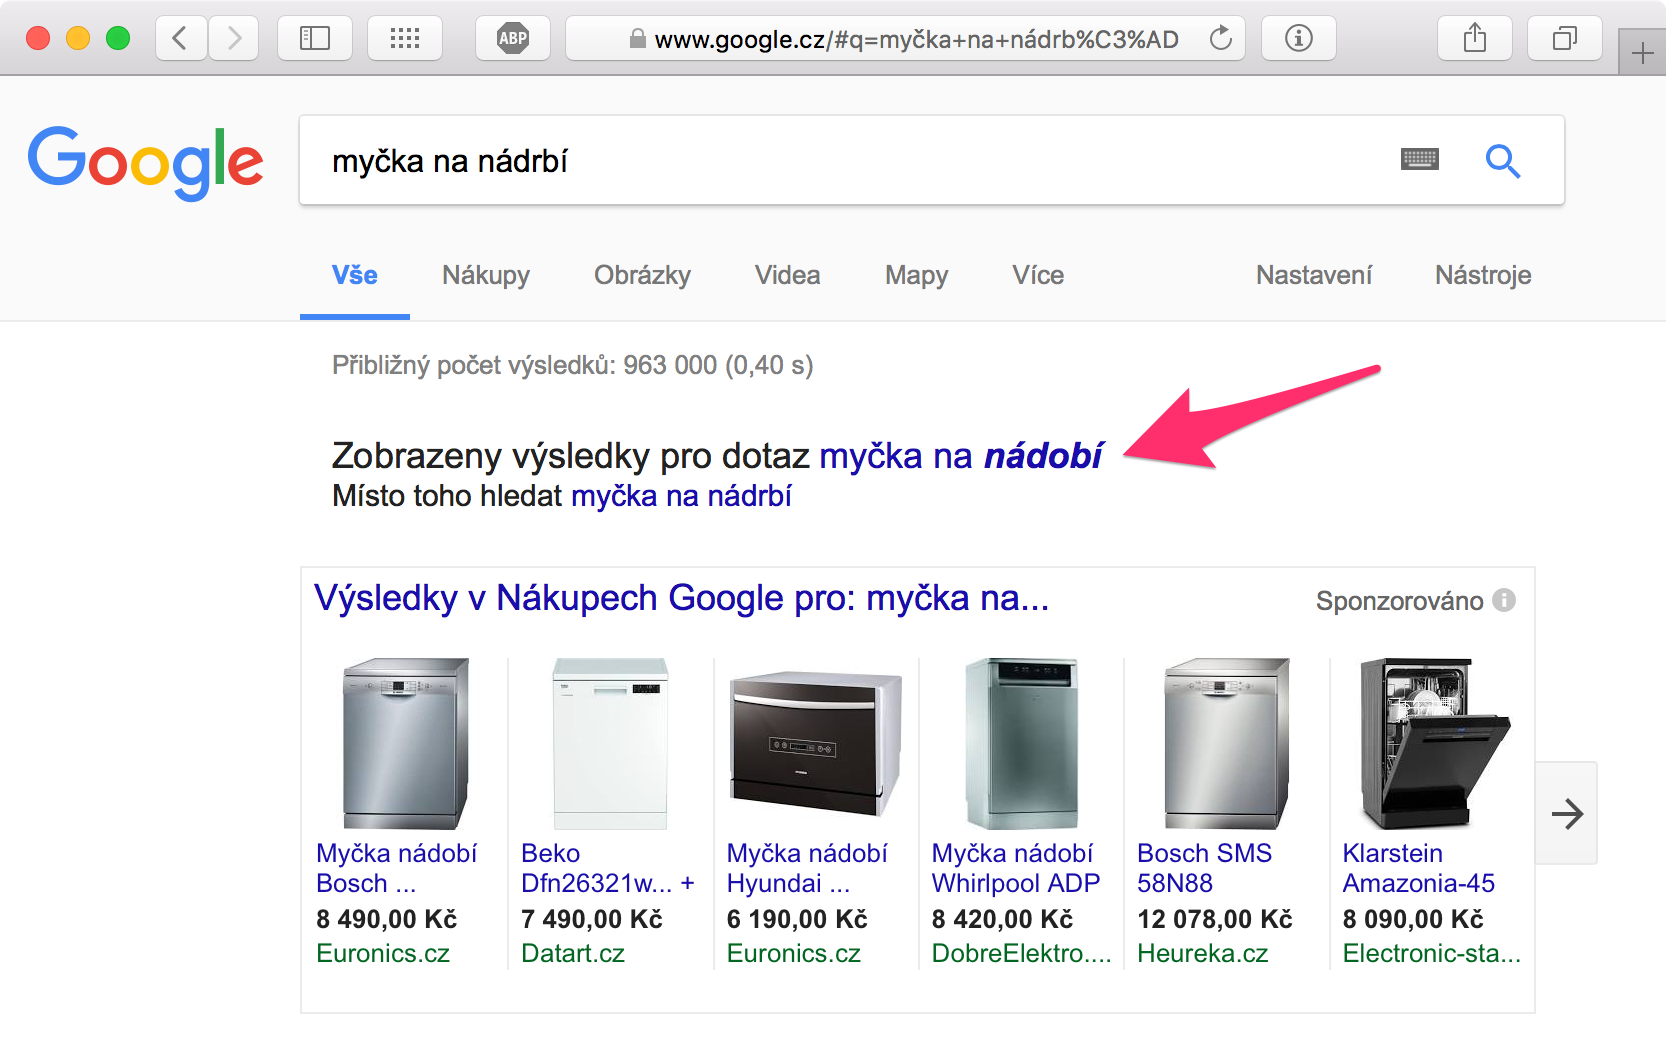
\includegraphics[width=\textwidth]{google-preklep.png}
\caption{Odhalení překlepu ve vyhledávání na webu google.com}
\label{google-preklep}
\end{figure}

U přibližného vyhledávání je třeba se vypořádat s měrou, jak přibližný daný výraz
je vůči výryzu hledanému, což lze vyjádřit pomocí editační vzdálenosti. Přistoupit
k této problematice lze i jednoduším přístupem -- generováním n-gramů.

\subsection{Editační vzdálenost}

Editační vzdálenost je způsob, jak vyjádřit podobnost dvou textových řetězců. Je
vyjádřena jako celé číslo, které udává počet operací nutný pro transformaci z~jednoho
třetového řetězce na druhý. Editačních vzdáleností pro textové vyhledávání je více, 
podle toho, jaké operace na textovém řetězci umožňují.

V roce 1965 Vladimir Levenshtein definoval \textbf{Levenshteinovu vzdálenost} jako počet
změn jednotlivých znaků vedoucí k transformaci z jednoho textu na druhý \cite{es-fuzziness}. 
Konkrétně šlo o~úpravy:

\begin{itemize}
\item Nahrazení jednoho znaku jiným: \textbf{jxblko} \textrightarrow ~\textbf{jablko}
\item Vložení jednoho znaku: \textbf{jaxblko} \textrightarrow ~\textbf{jablko}
\item Odstranění jednoho znaku: \textbf{jblko} \textrightarrow ~\textbf{jablko}
\end{itemize}

Frederick Damerau ji později rozšířil o další transformaci, která shodnou váhu:

\begin{itemize}
\item Prohození dvou znaků: \textbf{jbalko} \textrightarrow ~\textbf{jablko}
\end{itemize}

Tato transformace vlastně nahrazuje více dílčích operací definovaných výše. 
Vzdálenost s touto transformací o hodnotě 1 je označována jako 
\textbf{Damerau–Levenshteinova vzdálenost}. 
Počtem transformací se zvyšuje editační vzdálenost a zároveň
s~ní se snižuje pravděpodobnost, že daný textový řetězec je překlepem
druhého řetězce. Damerau vypozoroval, že 80\% překlepů má editační vzdálenost 
rovnou jedné \cite{damerau}. Je tedy výrazně nižší pravděpodobnost, že 
v textu bude tolik chyb, aby byla vzdálenost vyšší, což lze zohlednit při konstrukci
vyhledávacího algoritmu a bude mít zřejmě pozitivní vliv na rychlost vyhledávání.

Další vzdáleností je \textbf{Hammingova vzdálenost}, která počítá pouze s náhradou
znaku v textovém řetězci. Z tohoto omezení je však patrné, že je použitelná pouze pro 
řetězce shodné délky. V praxi textového vyhledávání tedy budeme pracovat pravděpodobně
s~vzdálenostmi definovanými výše.

Na mírně odlišném principu funguje \textbf{vzdálenost nejdelšího společného podřetězce}
(nebo také posloupnosti -- LCS distance). Jejím úkolem je nalézt nejvyšší možný za sebou
jdoucí počet znaků, který je společný oběma řetězcům. Tento přístup je ale méně
chodný pro vyrovnýní se s chybami uprostřed slov, navíc je výpočetně náročnější.

Další z možných vzdáleností je \textbf{Jarova vzdálenost}, která kromě počtu
změn na znacích počítá i počet shodných vzdáleností. Jejím rozšířením je
\textbf{Jaro-Winklerova vzdálenost}, která navíc počítá s~tím, že shodnost 
na~začátku řetězce má vyšší váhu, než na jeho konci -- vychází
totiž z pozorování, že na začátku textu se vyskytuje méně chyb \cite{christen}.
Tento přístup také dosahuje lepších výsledků u krátkých slov.

\subsection{N-gramová podobnost}

Vytváření n-gramů je používáno při indexaci, kdy jsou slova dělena na části dlouhé \verb|n| znaků.
Pokud bychom měli vygenerovat n-gramy o délce 3 (trigramy) pro slovo \textbf{telefon}, byly by 
to výrazy: \textbf{tel}, \textbf{ele}, \textbf{lef}, \textbf{efo} a \textbf{fon}. Lze si 
všimnout, že jednotlivé vygenerované výrazy se překrývají. Pokud pak uživatel zadá jako hledaný 
výraz \textbf{telef}, bude odpovídat trigrmům \textbf{tel}, \textbf{ele} a \textbf{lef}, 
tedy třem z celkem pěti. Trigramy jsou společně s digramy (n-gramy o délce dvou znaků) nejvhodnější
vzhledem k obvyklé délce slov. N-gram o délce 1 pak ztrácí smysl výše nastíněné logiky.

Porovnávání slov pomocí n-gramů je znázorněno na~následujícím schématu. Zde je zadané slovo
rozděleno na trigramy, z nichž každý je dále porovnávám s trigramy indexovaných slov.

\begin{figure}[h]
\center
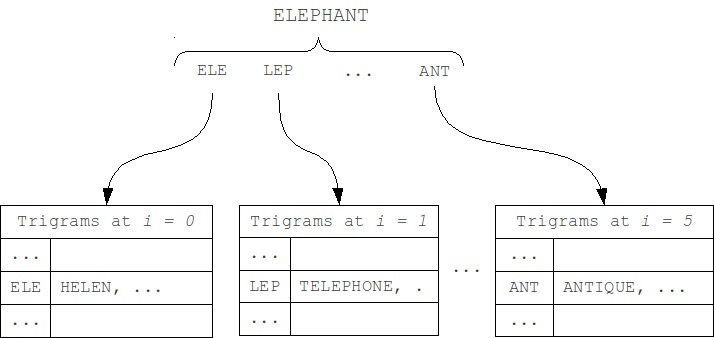
\includegraphics[width=\textwidth]{n-gram.png}
\caption{Vyhledávání pomocí n-gramů}
\label{n-gram}
\end{figure}

Tento mechanismus lze použít pro našeptávání i pro odhalení překlepů. Je snadno implementovatelný
a poměrně rychlý, selhává však u~překlepů v krátkých slovech \cite{n-gram}. Předpokládejme slovo 
o~délce 5 znaků -- \textbf{mobil}. Vzniklé trigramy jsou \textbf{mob}, \textbf{obi}, \textbf{bil}.
Pokud uživatel vyhledá slovo s překlepem přesně uprostřed (\textbf{movil}), nebude nalezena
shoda v žádném trigramu. 

Řešením by mohlo být snížení počtu znaků v n-gramu, což může na druhou stranu mít negativní 
vliv na~rychlost. Možným kompromisem tak může být různá délka n-gramů, kdy by vznikly kratší
n.gram pro začátek a konec slov. Konkrétně pro slovo \textbf{mobil} by tak vznikly n-gramy 
\textbf{m}, \textbf{mo}, \textbf{mob}, \textbf{obi}, \textbf{bil}, \textbf{il}, \textbf{l}.

\section{Relevance}

Relevancí rozumíme míru, jakou odpovídá nalezený dokument zadanému zadanému dotazu.
Je použitelná pro řazení nalezených dokumentů, kdy jsou nejprve zobrazeny dokumenty
více odpovídající hledanému výrazu. Dále je možné se na základě relevance rozhodnout, 
zda ještě nalezený dokument hledanému výrazu odpovídá, zda je vůbec třeba jej zobrazit.

Relevance je do jisté míry subjektivní, protože každý zákazník vyhledává na webu
s~jiným očekáváním, přestože třeba vyhledáva pomocí stejných výrazů. Objektivně lze však
relevanci vyjádřit pomocí TF-IDF, tedy frekvence nalezených výrazů vůči jejich frekvenci
v invertovaném indexu. 

V praxi elektronických obchodů však často do řazení
vstupují další veličiny, jako je cena produktu, skladovost nebo výše marže.
Pokud například uživatel vyhledá \textbf{iPhone}, může být žádoucí nejprve zobrazit
produkt \textbf{iPhone SE 64GB Vesmírně černý}, než jeho příslušenství, například
\textbf{Sportovní obal na iPhone SE} z důvodu několikanásobně vyšší marže na tomto produktu.

Elektronické obchody často také operují s akčním zbožím. Zejména v České republice je
obchodování se zlevněným zbožím populární, může bý tak žádoucí zobrazit takové produkty
dříve, než produkty prodávané za standardní cenu.

\begin{figure}[h]
\center
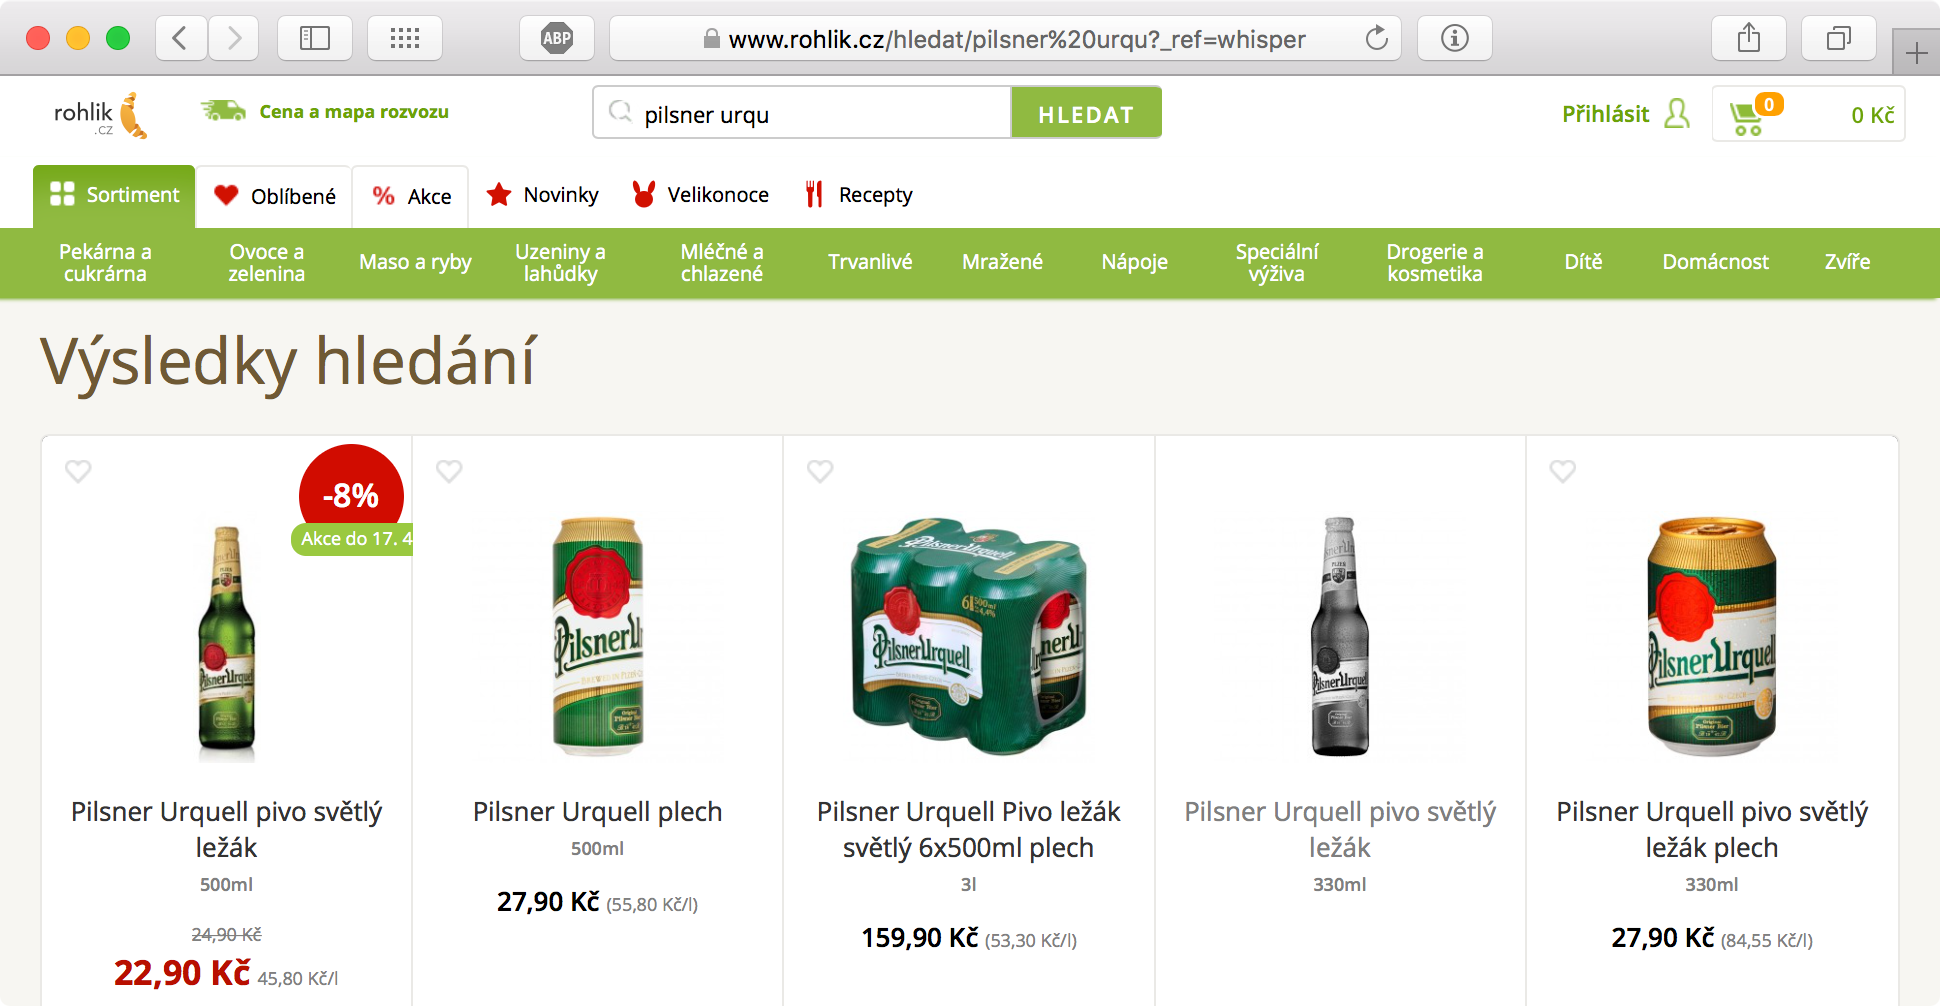
\includegraphics[width=\textwidth]{relevance.png}
\caption{Řazení výsledků -- upřednostnění akčního zboží}
\label{relevance}
\end{figure}

Pořadí výsledků nemusí být ovlivňováno jen zájmy provozovatele, mohou jej formovat
sami zákazníci svým chováním. Konkrétně v případě vyhledávání lze pozorovat proklikovost
jednotlivých produktů vzhledem k zadanému dotazu. Pokud se ukáže, že na základě
daného dotazu zákazníci nejčastěji klikají na konkrétní produkt, je možné jej zobrazit 
ve výsledcích vyhledávání pro tento dotaz dříve. 

S tímto přístupem je však možné jít ještě dál a začít vytvářet uživatelské profily zákazníků podle toho, 
o jaké zboží se zajímají, co vyhledávájí, jaké jsou jejich údaje zadané při registraci a objednávce 
(lokalita, pohlaví), nebo v jaké časy nakupují prostřednictvím jakých zařízení. Tato problematika je již
složitější, nicméně v posbíraných datech a vytvořených uživatelských profilech lze hledat další 
souvislosti pomocí statistických metod a strojového učení. Konkrétně lze zákazníka zařadit do určité 
skupiny pomocí shlukové analýzy a podle toho k němu přistupovat (upravit řazení výsledků vyhledávání) 
nebo využít algoritmů doporučovacích systémů.

Samotné řazení všech uložených dokumentů může být výpočetně náročné, v tu chvíli lze řadit
dokumenty ve dvou průchodech. V prvním průchodu jsou nalezeny dokumenty odpovídající zadanému 
dotazu a případně jřazeny s pomocí nenáročného výpočtu. Poté lze provést druhé řazení nad výběrem 
prvních dokumentů. Díky tomu, že už probíhá řazení nad malou množinou dat, je možné využít 
výpočetně náročnějších algoritmů.


%%%%%%%%%%%%%%%%%%%%%%%%%%%%
\chapter{Návrh řešení}

V této kapitole vytvářím návrh aplikace umožňující implementaci plnotextového vyhledávání
do elektronického obchodu, které bude možné provozovat jako službu. 

\section{Definice případů užití}
- Uzivatel zada XML\\
- Uzivatel vyhleda\\
- ...

\section{Návrh architektury aplikace}
- Frontend vs backend (API)...

\section{Návrh API}
- Frontend vs backend (API)...

% ...


%%%%%%%%%%%%%%%%%%%%%%%%%%%%
\chapter{Implementace}
- Vyber technologii a nastroju (jazyk, framework...), programovani...

\section{Výběr nástroje pro vyhledáváni}
- Popis a porovnani vhodnych nastroju\\
\hspace*{5mm}- MySQL\\
\hspace*{5mm}- Elasticsearch\\
\hspace*{5mm}- Sphinx\\
\hspace*{5mm}- ...

\section{Nastavení a nasazení Elasticsearch}
- Implementace indexace\\
- Implementace vyhledavani

\section{Výběr nástroje pro backend}
- Popis a porovnani vhodnych nastroju\\
\hspace*{5mm}- Go\\
\hspace*{5mm}- PHP\\
\hspace*{5mm}- Java\\
\hspace*{5mm}- ...

\section{Backend}
- Popis trid, rozhrani, implementacni detaily

\section{Frontend}
- Frontend: UI, komunikace s backendem

\section{Deployment}
- Deployment, CI

\section{Testování, ověření}
- Overeni funkcnosti a prinosu\\
- Testovani, zda jsou splnena akceptacni kriteria\\
- Porovnani s stavajicim resenim vyhledavani na konkretnim priklade


%%%%%%%%%%%%%%%%%%%%%%%%%%%%
\chapter{Závěr}
V této diplomové práci jsem...

\section{Dosažení vytčených dílů}
...

\section{Diskuze možného budoucího rozšiřování}
...


%%%%%%%%%%%%%%%%%%%%%%%%%%%%
\begin{thebibliography}{Mm99}

\bibitem{e-commerce} SUCHÁNEK Petr. \emph{E-commerce}.
Vyd.~1. Praha: Ekopress, s.r.o., 2012 144~s. ISBN 978-80-86929-84-2.

\bibitem{strossa} STROSSA, Petr. \emph{Počítačové zpracování přirozeného jazyka}.
Vyd.~1. Praha: Oeconomica, 2011 316~s. ISBN 978-80-245-1777-3.

\bibitem{searching} AYSE Göker a DAVIES John.
\emph{Information Retrieval: Searching in the 21st Century}.
Vyd.~1. Library of Congress Cataloging-in-Publication Data, 2009 295~s. ISBN: 978-0-470-02762-2.

\bibitem{mining} AGGARWAL Charu C., ZHAI ChengXiang. \emph{Mining Text Data}.
Springer New York Dordrecht Heidelberg London, 2000 522~s. ISBN 978-1-4614-3222-7.

\bibitem{api} STURGEON Phil. \emph{Build APIs You Won't Hate}.
Vyd.~1. Philip J. Sturgeon, 2015 188~s. ISBN 978-0692232699.

\bibitem{go-in-action} KENNEDY William. \emph{Go in Action}.
Manning Publications Co, 2016 264~s. ISBN 978-1-6172-9178-4.

\bibitem{es-guide} CLINTON Gormley, ZACHARY Tong. \emph{Elasticsearch: The Definitive Guide}.
O'Reilly Media, 2015 724~s. ISBN 978-1-4493-5854-9.

\bibitem{elastic-reference} Elasticsearch. \emph{Elasticsearch Reference} [online].
2017 [cit. 2017-03-03]. Dostupné z:
\url{https://www.elastic.co/guide/en/elasticsearch/reference/current/index.html}

\bibitem{algolia} Algolia. \emph{Hosted cloud search as a service} [online].
2017 [cit. 2017-03-03]. Dostupné z:
\url{https://www.elastic.co/guide/en/elasticsearch/reference/current/index.html}

\bibitem{swiftype} Swiftype. \emph{Site Search by Swiftype} [online].
2017 [cit. 2017-03-30]. Dostupné z: \url{https://swiftype.com/site-search}

\bibitem{cloud-search} AWS. \emph{Amazon CloudSearch} [online].
2017 [cit. 2017-03-30]. Dostupné z: \url{https://aws.amazon.com/cloudsearch/}

\bibitem{gse} Google. \emph{Custom Search Engine} [online].
2017 [cit. 2017-03-30]. Dostupné z: \url{https://cse.google.com/cse/}

\bibitem{amazon-100ms} GigaSpaces Blog.
\emph{Amazon found every 100ms of latency cost them 1\% in sales} [online]. \\
2017 [cit. 2017-03-26].
Dostupné z: \url{https://blog.gigaspaces.com/amazon-found-every-100ms-of-latency-cost-them-1-in-sales/}

\bibitem{stackshare-algolia} StackShare, Inc. 
\emph{How Algolia Reduces Latency For 21B Searches Per Month} [online].\\
2017 [cit. 2017-04-05]. Dostupné z:
\url{https://stackshare.io/algolia/how-algolia-reduces-latency-for-21b-searches-per-month}

\bibitem{postgres} PostgreSQL: Documentation. \emph{Full Text Search} [online].\\
2017 [cit. 2017-03-26]. Dostupné z: \url{https://www.postgresql.org/docs/9.5/static/textsearch.html}

\bibitem{lucene} The Apache Software Foundation. \emph{Apache Lucene} [online].\\
2017 [cit. 2017-03-26]. Dostupné z: \url{https://lucene.apache.org}

\bibitem{netmonitor} Sdružení pro internetový rozvoj. \emph{NetMonitor} [online].
2017 [cit. 2017-04-01]. Dostupné z: \url{http://www.netmonitor.cz}

\bibitem{xml-heureka} Heureka Shopping s.r.o. \emph{Specifikace XML souboru} [online].\\
2017 [cit. 2017-04-01]. Dostupné z: \url{https://sluzby.heureka.cz/napoveda/xml-feed/}

\bibitem{xml-zbozi} Seznam.cz, a.s. \emph{Specifikace XML feedu pro internetové obchody} [online].\\
2017 [cit. 2017-04-01]. Dostupné z:
\url{https://napoveda.seznam.cz/cz/zbozi/specifikace-xml-pro-obchody/specifikace-xml-feedu/}

\bibitem{nejpouzivanejsi-slova} TĚŠITELOVÁ Marie. \emph{O češtině v číslech}.
Praha: Academia, 1987 205~s.

\bibitem{es-fuzziness} Elasticsearch. \emph{The Definitive Guide - Fuzziness} [online].
2017 [cit. 2017-03-08]. Dostupné z:
\url{https://www.elastic.co/guide/en/elasticsearch/guide/current/fuzziness.html}.

\bibitem{damerau} DAMERAU, Fred J. \emph{A Technique for Computer Detection and Correction of Spelling Errors}.
Communications of the ACM (ACM), 1964, s. 171–176. ISSN 0001-0782. doi: 10.1145/363958.363994.
Dostupné z: \url{http://doi.acm.org/10.1145/363958.363994}

\bibitem{n-gram} SMETANIN Nikita. \emph{Fuzzy string search} [online].
2017 [cit. 2017-03-08]. 
Dostupné z: \url{http://ntz-develop.blogspot.cz/2011/03/fuzzy-string-search.html}.

\bibitem{christen} CHRISTEN, Peter. \emph{A Comparison of Personal Name Matching: Techniques and Practical Issues}.
ICDMW '06 Proceedings of the Sixth IEEE International Conference on Data Mining, 2006, s. 290-294,
IEEE Computer Society Washington, DC, USA. doi: 10.1145/363958.363994. 
Dostupné z: \url{http://users.cecs.anu.edu.au/~Peter.Christen/publications/tr-cs-06-02.pdf}. 
ISBN: 0-7695-2702-7.

\end{thebibliography}


%%%%%%%%%%%%%%%%%%%%%%%%%%%%
\chapter*{Rejstřík}
...


%%%%%%%%%%%%%%%%%%%%%%%%%%%%
\appendix

\chapter{Obsah přiloženého DVD}

\begin{itemize}
\item Soubor Diplomova\_prace\_2017\_Ludek\_Vesely.pdf
\begin{itemize}
	\item Text diplomové práce
\end{itemize}

\end{itemize}


%\chapter{Graf jako příloha}
%\begin{figure}[h]
%\center
%
\includegraphics[width=0.86\textwidth]{todo.pdf}
%\end{figure}


%%%%%%%%%%%%%%%%%%%%%%%%%%%%
\end{document}
